\subsection{Longest common sub-sequence (LCS)}
Given two String $x$ and $y$. Find the longest common sub-sequence between $x$ and $y$.
 
\begin{center}
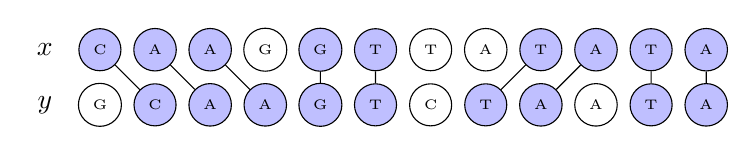
\begin{tikzpicture}[scale = 0.7]
\node at (-1, 1) {$x$};
\node at (-1, 0) {$y$};

\node[draw, circle] at (0, 0) (A)                  {\tiny G};
\node[draw, circle, fill = blue!25] at (1, 0) (B)  {\tiny C};
\node[draw, circle, fill = blue!25] at (2, 0) (C)  {\tiny A};
\node[draw, circle, fill = blue!25] at (3, 0) (D)  {\tiny A};
\node[draw, circle, fill = blue!25] at (4, 0) (E)  {\tiny G};
\node[draw, circle, fill = blue!25] at (5, 0) (F)  {\tiny T};
\node[draw, circle] at (6, 0) (G)                  {\tiny C};
\node[draw, circle, fill = blue!25] at (7, 0) (H)  {\tiny T};
\node[draw, circle, fill = blue!25] at (8, 0) (I)  {\tiny A};
\node[draw, circle] at (9, 0) (J)                  {\tiny A};
\node[draw, circle, fill = blue!25] at (10, 0) (K) {\tiny T};
\node[draw, circle, fill = blue!25] at (11, 0) (L) {\tiny A};

\node[draw, circle, fill = blue!25] at (0, 1) (a)  {\tiny C};
\node[draw, circle, fill = blue!25] at (1, 1) (b)  {\tiny A};
\node[draw, circle, fill = blue!25] at (2, 1) (c)  {\tiny A};
\node[draw, circle] at (3, 1) (d)                  {\tiny G};
\node[draw, circle, fill = blue!25] at (4, 1) (e)  {\tiny G};
\node[draw, circle, fill = blue!25] at (5, 1) (f)  {\tiny T};
\node[draw, circle] at (6, 1) (g)                  {\tiny T};
\node[draw, circle] at (7, 1) (h)                  {\tiny A};
\node[draw, circle, fill = blue!25] at (8, 1) (i)  {\tiny T};
\node[draw, circle, fill = blue!25] at (9, 1) (j)  {\tiny A};
\node[draw, circle, fill = blue!25] at (10, 1) (k) {\tiny T};
\node[draw, circle, fill = blue!25] at (11, 1) (l) {\tiny A};

\draw (B) edge (a);
\draw (C) edge (b);
\draw (D) edge (c);
\draw (F) edge (f);
\draw (H) edge (i);
\draw (I) edge (j);
\draw (K) edge (k);
\draw (L) edge (l);
\draw (E) edge (e);

\end{tikzpicture}
\end{center}

\begin{itemize}
 \item \textbf{Formulation:}
$lcs[i][j] =$ size of \\\text{\ \ \ } $LCS(x[0] x[1] \cdots x[i - 1], y[0] y[1] \cdots y[j - 1])$
  \item \textbf{Base case:} $
lcs[0][j]  = 0$ \hspace{15pt} 
$lcs[i][0]  = 0$
  \item \textbf{Other cases: }
  \begin{itemize}
  \item Si $x[i-1] = y[i-1]$ alors: \\
  \quad $lcs[i][j] = 1 + lcs[i-1][j-1]$ 
  \item Si $x[i-1] \neq y[i-1]$ alors: \\
  \quad $lcs[i][j] = \max \{lcs[i-1][j], lcs[i][j-1]\}$
  \end{itemize}
\end{itemize}